\chapter{Определение траектории движения материальной точки в движущемся
центрально-симметричном поле сил. Дифференциальное уравнение траектории
движения. Уравнение Бине. Решение уравнения Бине. Виды траекторий. Влияние
начальных условий на вид траектории.}


Поле называется \textit{центральным}, если его линии - пучок прямых выходящих
из точки \( O \)(центра). Если центральное поле зависит только от расстояния от
точки наблюдения до \( O \), то оно называется \textit{центрально-симметричным}.
Если ввести радиус-вектор \( \vec{r} \) от точки \( O \) до точки наблюдения,
орт вдоль направления радиус-вектора \( \vec{e}_r \), модуль \( \vec{r} \)
обозначить \( r \), то центральное поле сил:
\[
    \vec{F} = F(r)\vec{e}_{r}.
\]

Уравнение движения материальной точки массой \( m \) примет вид: 
\[
    m\der{\vec{v}}{t} = m\dder{\vec{r}}{t} = F(r)\vec{e}_{r}.
\]
    
Момент количества движения относительно точки \( O \)
\( \vec{L} = m \vec{v} \times \vec{r} \), рассмотрим производную:
\[
    \der{\vec{L}}{t} = 
    m \der{\vec{v}}{t} \times \vec{r} + m \vec{v} \times \der{\vec{r}}{t} =
    F(r)\vec{e}_{r} \times \vec{r} + m \vec{v} \times \vec{v} = 0.
\]
    
Это значит, что момент количества движения сохраняется и движение происходит в
плоскости начальной скорости и радиус-вектора.

\sidefig(9cm)
{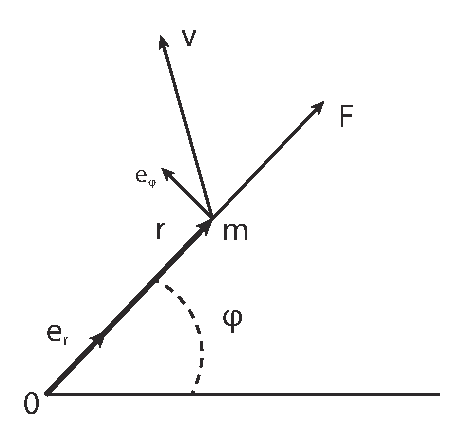
\includegraphics[ width=1\textwidth]{41}}{
В этой плоскости введём полярную систему координат, как показано на рисунке.
Тогда:
\[
    \vec{r} = r \vec{e}_{r},
\]
\[
    \der{\vec{r}}{t} = 
    \der{r}{t} \vec{e}_{r} + 
    r \der{\vec{e}_{r}}{t} =
    \der{r}{t} \vec{e}_{r} + 
    r \der{\phi}{t}\vec{e}_{\phi},
\]
\begin{gather*}
    \dder{\vec{r}}{t} = 
    \left(
        \dder{r}{t} - 
        r
        \left(
        \der{\phi}{t}
        \right)^2
    \right)\vec{e}_{r} + \\ +
    \left( 
        2\der{r}{t} \der{\phi}{t}+ 
        r \dder{\phi}{t}
    \right)\vec{e}_{\phi}.
\end{gather*}
}

Получаем систему уравнений движения:
\[
    \left\{
    \begin{array}{l}
        \dder{r}{t} - 
        r
        \left(
        \der{\phi}{t}
        \right)^2 = 
        F(r),
        \\ 
        2\der{r}{t} \der{\phi}{t}+ 
        r \dder{\phi}{t}
        =
        \frac{1}{r}
        \der{}{t}
        \left(
            r^2 \der{\phi}{t}
        \right)
        = 0.
    \end{array}
    \right.
\]
Величина \( \frac{1}{2}r^2 \der{\phi}{t} \) носит название
\textit{секториальной скорости}, т. е. производной по времени от площади,
описываемой радиус-вектором, а последнее уравнение показывает, что она
постоянна. Её постоянство эквивалентно постоянству момента количества движения
\( L \) относительно оси проведённой перпендикулярно плоскоcти движения через
точку \( O \). Связь между моментом количества движения и секториальной
скоростью:
\[
    \frac{1}{2}r^2 \der{\phi}{t} = \frac{L}{2m}.
\]
Это выражение носит название интеграла площадей. Исключим с его помощью \( t \)
из уравнений движения:
\[
    \der{r}{t} = 
    \der{r}{\phi} \der{\phi}{t} =
    \frac{L}{mr^2 } \der{r}{\phi} =
    -\frac{L}{m} \der{}{\phi}\left( \frac{1}{r} \right),
\]   
\[
    \dder{r}{t} = 
    \der{}{t}\der{r}{t}  =
    \der{}{\phi}\left(\der{r}{t}\right)\der{\phi}{t} =
    -\frac{L^2}{m^2 r^2 } \der{}{\phi^2}\left( \frac{1}{r} \right).
\]     
Тогда:
\[
    -\frac{L^2}{m^2 r^2 } \der{}{\phi^2}\left( \frac{1}{r} \right) -
    \frac{L^2}{m^2 r^3} = 
    F(r)
\]   
или
\[
    \der{}{\phi^2}\left( \frac{1}{r} \right) +
    \frac{1}{r} = 
    - F(r)\frac{m^2 r^2}{ L^2}.
\]   
Это уравнение называют \textit{уравнением Бине}. В частном случае кулоновых
полей:
\[
    F(r) = -\frac{\alpha}{r^2}
\]   
оно переходит в
\[
    \der{}{\phi^2}\left( \frac{1}{r} \right) +
        \frac{1}{r} = 
        \frac{m^2 \alpha}{ L^2}.
\]     
Его решения:
\[
    \frac{1}{r} = A \cos (\phi - \theta) + \frac{m^2 \alpha}{ L^2}.
\]   
    
Если нам известны начальные условия \( r_0 \), \( \phi_0 = 0 \), \( v_0 \)
и угол между вектором \( \vec{r}_{0} \) и начальной скоростью \( \gamma \), то
можно найти константы \( A \) и \( \theta \).
\[
    \left.\der{r}{\phi}\right|_{t=0} = 
    \left.\frac{\der{r}{t}}{\der{\phi}{t}}\right|_{t=0} =
    \frac{ v_0 \cos \gamma}{\frac{v_0}{r_0}  \sin \gamma} =
    \frac{ r_0 \cos \gamma}{ \sin \gamma},
\]
\[   
    L = r_0 v_0 \sin \gamma,
\]
\[   
    \der{}{\phi}\frac{1}{r} = \frac{1}{r^2} \der{r}{\phi} =
    A \sin (\phi - \theta).
\]
    
Для \( A \) и \( \theta \) получаем систему:
\[
    \left\{\begin{array}{l}
        \frac{1}{r_0} -  \frac{m^2 \alpha}{ L^2} = A\cos\theta, \\
        \frac{ \cos\gamma}{ r_0 \sin\gamma} = - A\sin\theta.
    \end{array}\right.
\]
    
Тогда:
\[
    A = 
        \sqrt{\left
        (\frac{1}{r_0} -  \frac{m^2 \alpha}{ L^2}
        \right)^2+
        \frac{ \ctg^2 \gamma}{ r_0^2}},
\]   
\[
    \theta = \arctg\frac{\ctg\gamma}{r_0}.
\]   

Если ввести новый угол \( \omega = \phi - \theta \), называемый истинной
аномалией, и постоянные \( e = A\frac{L^2}{m^2 \alpha} \) и
\( p = \frac{L^2}{m^2 \alpha} \), то уравнение траектории примет вид
канонического уравнения конического сечения:
\[
    r = \cfrac{p}{1+e \cos \omega}.
\]   

Если \( e < 1 \), то траекторией будет эллипс, \( e = 1 \) -- парабола,
\( e > 1 \) -- гипербола.

\newpage
